\chapter{Sistemas imunológicos artificiais}

O estudo sobre os Sistemas Imunológicos Artificiais (um subcampo da área de Inteligência Computacional) iniciou no início dos anos 90, baseado na proposição de aplicar modelos teóricos da Imunologia a problemas de aprendizagem de máquina e automação.

Os primeiros trabalhos basearam-se em paradigmas como o das Redes Imunológicas Artificiais, os Algoritmos Genéticos, Aprendizagem por Reforço e Sistemas de Classificação. Os primeiros trabalhos a formarem uma identidade própria desses algoritmos foram aqueles que relacionavam o sistema imunológico como uma analogia aos sistemas computacionais de proteção da informação, como \citet{Forrest1994} e \citet{Forrest1997}.

Os algoritmos modernos são inspirados em algoritmos de três campos principais: seleção clonal, seleção negativa e redes imunológicas. Esse tipo de sistema é comummente aplicado a problemas de detecção de padrões, classificação, otimização, \emph{clustering} e outros domínios de aprendizagem de máquina.

A última década mostrou um grande aumento no interesse pelos algoritmos baseados em sistemas imunológicos, conforme apresentado em \citet{Dasgupta2010}, por serem uma boa fonte de inspiração para novas abordagens para solução de problemas complexos. O sistema imunológico natural oferece metáforas ricas pelo fato de ser um sistema altamente distribuído, adaptativo e auto-organizável, além de suas capacidades de aprendizado, memorização, extração de características e reconhecimento de padrões.

Esse artigo contém uma lista de diversos trabalhos recentes na área de Sistemas Imunológicos Artificiais. A tabela \ref{ais:recent} apresenta uma lista dos algoritmos, além do número de trabalhos apresentados.

\vspace{2mm}
\begin{table}[h!]
    \centering
    \caption{Trabalhos recentes na área de Sistema Imunológico Natural \cite{Dasgupta2010}}
    \begin{tabular}{l c r}
        \hline
        Algoritmos & Trabalhos   \\
        \hline
        Seleção negativa    & 27 \\
        Abordagens híbridas & 18 \\
        Células dendríticas & 14 \\
        Redes imunológicas  & 10 \\
        Teoria do Perigo    & 8  \\
        Seleção clonal      & 5  \\
        Outros modelos      & 3  \\
        \hline
    \end{tabular}
    \label{ais:recent}
\end{table}
\vspace{2mm}

\section{Algoritmos}

Em \citet{Dasgupta2010}, os autores apresentam pesquisas recentes na área de Sistemas Imunológicos Artificiais, e mostram que as pesquisas recentes nessa área têm se focado em quatro algoritmos principais. Esse algoritmos são: (1) seleção negativa, (2) redes imunológicas artificiais, (3) seleção clonal e (4) Teoria do Perigo e algoritmos de células dendríticas, e serão apresentados nas seções seguintes.

\subsection{Seleção negativa}

Forrest et al \cite{Forrest1994} publicou um artigo chamado "Self-Nonself Discrimination in a Computer" (Discriminação do Próprio-Não-Próprio em um Computador), que propunha um método chamado de \emph{algoritmo de seleção negativa}. Esse algoritmo é baseado na capacidade de discriminação entre o próprio e o não-próprio no sistema imunológico adaptativo através do processo de seleção negativa na geração de células T no sistema imunológico. Foi projetado para aplicações de detecção de alteração, detecção de intrusão e outros problemas de reconhecimento de padrões e classificação binária, e foi aplicado inicialmente a um problema de detecção de vírus de computador.

 O princípio da técnica da seleção negativa é a modelagem do que é desconhecido como um complemento do que é conhecido. Isso é conseguido através de um processo contínuo de seleção negativa, que elimina células que reajam a células próprias. No sistema imunológico natural, as precursoras das células T deslocam-se da medula óssea para o timo, onde ocorre o seu desenvolvimento. As células proliferam-se e diferenciam-se, através de mutação genética. A seleção negativa é aplicada sobre aquelas células T que são ativadas por células próprias. Os algoritmos baseados na seleção negativa são baseados nesse comportamento, e suas principais características são a representação negativa da informação, geração distribuída do conjunto de detectores e classificação dos dados em apenas uma classe.

A representação dos dados é um dos principais aspectos desse algoritmo: geralmente são usados \emph{strings} ou vetores de valores reais. Existe também uma regra de combinação particular de cada algoritmo, tipicamente baseada em distância ou alguma medida similar. Muitas variações desse algoritmo foram desenvolvidas, mas todas compartilham essas características básicas.

\subsection{Redes imunológicas artificiais}

Redes imunológicas artificiais (\emph{Artifial immune networks}, AINs) são inspiradas no modelo de redes imunológicas de Farmer et. al \cite{Farmer1986}, e foram propostas por \cite{Ishida1990}. \cite{Timmis2000} redefiniu e reimplementou a rede imunológica artificial, e esses trabalhos foram nomeados conjuntamente como AINEs (\emph{Artificial Immune NEtworks}, Rede Imunológicas Artificiais). Uma rede imunológica artificial consiste de um conjunto de células B e ligações entre essas células. Essas redes permitem ao sistema imunológico ter uma memória imunológica: as células estimulam ou reprimem umas às outras, atingindo uma memória estável. Sua utilização é ampla em campos como a mineração de dados e aprendizagem de máquina. 

O sistema proposto por \citeauthor{Timmis2000} era composto de uma medula óssea, uma rede de células B e uma população de antígenos. A população de células B é inicializada aleatoriamente e, uma a uma, são inseridas em um ponto também aleatório na rede. Caso a célula seja capaz de ligar-se à população de antígenos, clones das células B são gerados, e aqueles com maior afinidade com as células da rede são mantidos. Os algoritmos de redes imunológicas artificiais incorporaram algumas ideias das teorias da seleção clonal: as células B nas AINE sofrem clonagem, mutação e seleção quando são estimuladas pela rede.

\subsection{Seleção clonal}
\label{sec:ais_clonalg}

Em 2000, Castro et al.\cite{Castro2000} propôs o algoritmo de seleção clonal (CSA), mais tarde conhecido como CLONALG. Esse algoritmo é baseado nos princípios da imunidade adquirida de seleção clonal e maturação de afinidade, que são por sua vez baseados nos princípios da teoria de Darwin da seleção natural.

Segundo a teoria da seleção clonal, quando um linfócito identifica um antígeno, ele prolifera, criando milhares de cópias de si mesmo, e diferenciando-se em diferentes tipos de células: de plasma e de memória.

Células de plasma têm vida curta, e produzem grandes quantidades de anticorpos moleculares. Células de memória vivem por um longo período, fazendo parte das respostas secundárias caso o antígeno venha a ser identificado novamente.

A clonagem de células B causam um aumento na afinidade do antígeno que causou a clonagem, através de um processo denominado maturação de afinidade. Esse processo é composto de duas partes: hipermutação somática, que diversifica os anticorpos introduzindo mudanças aleatórias nas novas gerações; e um mecanismo de seleção, que garante que apenas os clones com maior afinidade sobrevivam. Assim, uma geração de células inclui a inicialização de soluções candidatas, seleção, clonagem, mutação, reseleção e substituição de população, semelhante a um algoritmo genético (GA).

A parte essencial dessa teoria é que, quando um linfócito é clonado, sofre pequenas alterações em sua estrutura (hipermutação somática), que alteram seus receptores e sua capacidade de reconhecimento, assim como os anticorpos que são gerados por ele. Assim, essa teoria sugere que um repertório inicial de células imunes genéricas é capaz de evoluir para responder a mudanças no ambiente, sem ter informações detalhadas sobre os agentes que compõem esse ambiente.

\subsection{Teoria do Perigo}

No primeiro artigo a propor a aplicação da Teoria do Perigo em um sistema computacional, \citeauthor{Aickelin2002} apresentam como a Teoria do Perigo pode auxiliar na aplicação de sistemas imunológicos artificiais em problemas complexos de detecção de anomalia, citando algumas analogias dos sistemas imunológicos presentes na Teoria do Perigo:

\begin{enumerate}[a)]
    \item Uma APC é necessária para apresentar o sinal de perigo.
    \item O "sinal de perigo" pode não ter relação nenhuma com perigo.
    \item O sinal de perigo pode ser positivo (presença de sinal) ou negativo (ausência de sinal).
    \item Uma medida de proximidade pode ser usada para simular uma zona de perigo.
    \item Uma resposta imunológica não deve gerar novos sinais de perigo.
\end{enumerate}

Segundo a teoria do perigo, a resposta imunológica é desencadeada por sinais de perigo. Representações dos sinais de perigo podem incluir uso anormal de memória, atividade de disco imprópria, etc. O sistema imunológico reage aos antígenos dentro de uma zona de perigo centrada no local da origem do sinal, que pode ser modelada como uma medida de similaridade ou relação de causalidade. Aqueles anticorpos que combinam-se aos antígenos (sinal um) dentro de uma zona de perigo (sinal dois) proliferam, gerando células de memória.

\subsection{Algoritmo de células dendríticas}

O algoritmo de células dendríticas é inspirado pela Teoria do Perigo, mais especificamente na função das células dendríticas. As células dendríticas foram identificadas por \citet{Steinman1973} e o seu principal papel é o de célula apresentadora de antígeno (APC). O objetivo do algoritmo de células dendríticas é preparar um conjunto de células dendríticas maduras que forneçam informações dependentes de contexto sobre como classificar como normais ou anômalos os padrões de entrada.

As células dendríticas encontram-se distribuídas em todos os tecidos e executam funções diferentes de acordo com o tecido em que atuam. Quando ainda estão em um estado de imaturidade viajam na corrente sanguínea, até que sofrem diferenciação e maturação quando propriamente estimuladas. Elas então migram para tecidos periféricos, onde apresentam antígenos para as células T, iniciando as respostas imunológicas. As células dendríticas são de três tipos principais:

\begin{description}
    \item[Imaturas]: coletam partes dos antígenos e sinais
    \item[Semi-maduras]: decidem que os sinais locais não representam perigo e apresentam um sinal de tolerância às céulas T
    \item[Maduras]: decidem que os sinais locais são de perigo e apresentam um sinal de reposta imune às células T
\end{description}

O primeiro algoritmo baseado no comportamento dessas células foi desenvolvido em \citet{Greensmith2005} e definido formalmente em \citet{Greensmith2006}. Esse algoritmo combina sinais múltiplos para estimar o estado corrente do ambiente e amostrar outro antígeno assincronamente. Sua execução consiste de três etapas principais: inicialização, atualização e agregação. A inicialização configura diversos parâmetros. A fase de atualização é dividida em uma fase de atualização do tecido, onde o valor dos sinais é calculado de acordo com os dados de entrada, resultando nos sinais de entrada das células, e uma fase de atualização das células. O último estágio da execução é a agregação: os antígenos coletados são analisados e classificados.

O algoritmo aplica pesos pré-definidos aos sinais de entrada para produzir três sinais de saída: sinal de coestimulação, sinal de semi-maturação e sinal de maturação. Se a soma dos valores dos sinais de maturação for maior que a somas dos sinais de semi-maturação, a célula é diferenciada para um estado maduro e tem assinalado um valor de contexto. O algoritmo calcula a proporção de valores de contexto maduro de um antígeno para o total de antígenos, chamada de MCAV (\emph{Mature Context Antigen Value}, Valor de Contexto Maduro do Antígeno), e aquelas antígenos cujo MCAV excede um limite pré-definido são classificados como anômalos.

\section{Implementação}

A modelagem de um problema como um sistema imunológico artificial requer a definição de quatro componentes: codificação, medida de similaridade, seleção e mutação. De maneira geral, o funcionamento de um sistema baseado no modelo imunológico é: uma vez que a \emph{codificação} e uma \emph{medida de similaridade} tenham sido escolhidas, o sistema executa a \emph{seleção} e \emph{mutação}, ambas baseadas na medida de similaridade, até que o critério de parada seja satisfeito \cite{Aickelin2005}. Essas quatro etapas são detalhadas nas próximas seções.

\subsection{Codificação}

A codificação é uma etapa essencial na definição de um Sistema Imunológico Artificial. Ela afeta toda modelagem do sistema, em especial a medida de similaridade, e pode ser responsável pelo seu sucesso ou falha. Os dois principais agentes do sistema imunológico, antígenos e anticorpos, são também os principais elementos que devem ser modelados. Eles são são comumente representados da mesma forma.

Um antígeno é uma parte do objetivo ou solução da aplicação, que pode ser único ou um parte de um conjunto-solução. Os anticorpos são o resto dos dados, e geralmente existem em grande quantidade. Em uma aplicação de detecção de intrusão, por exemplo, o antígeno poderia ser o conjunto de dados que define um tráfego de dados, e os anticorpos, os conjuntos de dados que já foram identificados como legais.

Na maioria dos problemas, a representação desses dois elementos é feita através de um vetor de números ou de características. Cada posição desse vetor representa uma característica da instância. Os tipos mais comuns de dados são números (inteiros ou reais), \emph{strings} e valores binários.

\subsection{Medida de similaridade}

A medidade de similaridade (também chamada de medida de afinidade, principalmente na área de Sistemas Imunológicos Artificiais) é usada para comparar duas instâncias, e mede o quanto uma é semelhante à outra. É usada principalmente para agrupar instâncias em grupos e nas condições de término (o algoritmo termina quando o modelo descreve as instâncias com uma medida de similaridade satisfatória, que varia de acordo com a aplicação, o tempo de execução e o nível de similaridade necessário).

Uma função de similaridade simples é o número de \emph{bits} que são idênticos nas duas sequências. Por exemplo, para os \emph{strings} (00011) e (00000), a função retornaria 3. Essa função é oposta à distância de Hamming, que mede quantos \emph{bits} devem ter seus valores trocados para tornar as sequências iguais. Em alguns problemas, essa medida não é suficiente, já que ela não tem a noção de continuidade. Uma alternativa é calcular o número de posições iguais contínuas, retornando o maior valor. Assim, o exemplo anterior também receberia o valor 3, mas as sequências (00000) e (01010) receberia 1. Essa diferenciação pode ter ser apropriada ou não, dependendo do problema. Para variáveis não-binárias, existem ainda mais possibilidades de medida de distância, como a distância Euclideana.

Para os problemas de mineração de dados, a aptidão geralmente significa correlação, e uma medida simples de correlação é o coeficiente de correlação de Pearson. A correlação de duas instâncias \emph{u} e \emph{v} é definida como:

\vspace{2mm}
\begin{equation}
r=\frac{
    \sum\limits_{i=1}^{n}
        (u_i-\overline{u})
        (v_i-\overline{v})
    }
    {\sqrt{
        \sum\limits_{i=1}^{n}
            (u_i-\overline{u})^2
        \sum\limits_{i=1}^{n}
            (v_i-\overline(v))^2
        }
    }
\end{equation}
\vspace{2mm}

Onde \emph{u} e \emph{v} são duas instâncias, \emph{n} é o número de variáveis comuns a u e v, \emph{$u_i$} é o valor da varável i na instância u e \emph{$\overline{u}$} é a média dos valores de todas as variáveis de u (não apenas das variáveis comuns a u e v). A média é modificada para que o valor 0 seja atribuído a instâncias sem nenhuma variável em comum. O resultado são valores de -1 a 1, onde 1 significa forte concordância e -1 forte discordância.

Para algumas aplicações, aptidão pode não ser benéfica, e as instâncias que são mais semelhantes são na verdade descartadas. Esse processo é conhecido como seleção negativa, e é equivalente ao processo que acredita-se que ocorre durante a maturação dos linfócitos B, onde eles aprendem a não identificar os tecidos próprias, para que não se inicie uma reação autoimune.

A seleção negativa é muito aplicada a sistemas de segurança. Cria-se um ambiente seguro, formado apenas por componentes confiáveis. Na inicialização do sistema, é gerado um grande número de detectores randômicos, que são aplicados aos dados gerados por esse ambiente. Aqueles que identificarem os dados legais são eliminados, restando ao final apenas aqueles que não identificarem. Esses detectores formarão o sistema de detecção, que irá monitorar constantemente o ambiente. Caso algum detector identifique os dados no ambiente, é gerado um alerta de "possível não-próprio".

A otimização da aptidão dos modelos em muitos casos não é realmente o objetivo do sistema se o objetivo é criar generalizações através de um subconjunto dos dados existentes \cite{Hand2001}. Um modelo com grande aptidão pode não se adaptar a novas instâncias que venham a ser analisadas pelo sistema.

\subsection{Seleção}

Nos Sistemas Imunológicos Artificiais, os três métodos de seleção mais usados são a seleção negativa, seleção clonal e seleção de vizinhança. O papel da seleção é explicado a seguir, no contexto do funcionamento do sistema. O estado inicial do sistema é vazio. O antígeno é então codificado (conforme a representação definida anteriormente) e adicionado ao sistema. Cada anticorpo é codificado e adicionado ao sistema, um a cada iteração. Os anticorpos iniciam com um determinado valor de concentração, que é análogo ao número de células presentes no sistema imunológico artificial. Esse valor é constantemente decrementado conforme o tempo passa, representando a morte natural de parte das células.

Anticorpos cuja concentração ultrapassa um certo limiar mínimo são removidos do sistema. Um anticorpo aumenta sua concentração de acordo com a sua similaridade com o antígeno. Quanto maior a similaridade, mais sua concentração aumenta, em um processo similar à expansão clonal que ocorre com as células imunológicas quando identificam um antígeno. Após todos os antígenos serem adicionados ao sistema, começa um processo iterativo de decremento de concentração e clonagem, até que o sistema entre em equilíbro: não ocorram remoções por um determinado período de tempo.

O trecho de código \ref{aisalg} mostra o pseudocódigo de um Sistema Imunológico Artificial.

\begin{lstlisting}[caption=Pseudo código de um Sistema Imunológico Artificial \cite{Aickelin2005},label=aisalg]
Inicializar o sistema
Codificar o antígeno Ag
ENQUANTO (Sistema não cheio) E (Ainda existem anticorpos) FACA
    Adicionar próximo anticorpo Ab
    Calcular a medida de similaridade entre Ag e Ab
    ENQUANTO (Sistema cheio) E (Sistema não estabilizado) FACA
        Reduzir a concentração de todos os Abs
        Estimular os Abs conforme a medida de similaridade
    FIMENQUANTO
FIMENQUANTO
\end{lstlisting}

\subsection{Mutação}

A mutação utilizada nos sistemas imunológicos é similar àquela encontrada em Algoritmos Genéticos. \emph{Strings} binárias têm seus dígitos invertidos, valores reais são alterados aleatoriamente e os outros tipos são trocados de posição. Além disso, geralmente usa-se a mutação somática, inspirada na reprodução de células do sistema imunológico, onde a mutação é mais severa conforme o grau de similaridade entre o anticorpo e o antígeno aumenta (ou diminui, caso esteja-se aplicando a seleção positiva). 

A estratégia de mutação deve ser planejada com cuidado, porque nem todas as técnicas funcionam para qualquer tipo de dados. \citet{Aickelin2005} utiliza o exemplo de um sistema de recomendação de filmes, onde uma base de dados é utilizada para recomendar filmes aos usuários, analisando usuários que recomendaram filmes semelhantes àqueles recomendados por ele. Nesse caso, não faria sentido aplicar algum tipo de mutação: ao fim, os anticorpos convergiriam para o próprio usuário.

Mesmo assim, a mutação pode ser muito útil quando aplicada a alguns problemas, como detecção de intrusão e mineração de dados \cite{DeCastro2002}. 

\section{Espaço de formas}

Os formalismos do espaço de formas e topologia de afinidade são dois paradigmas geométricos populares, originados na imunologia teórica e computacional, muito utilizados em aplicações recentes do campo de sistemas imunológicos artificiais \cite{Brownlee2007}. \citeauthor{Perelson1979} apresentaram o formalismo do espaço de formas em \citet{Perelson1979}, onde os autores fizeram uma investigação teórica das diferentes formas e capacidades de reconhecimento dos anticorpos. As ideias apresentadas nesse trabalho influenciara muitos trabalhos no fim dos anos 80 e início dos anos 90, principalmente em trabalhos teóricos sobre seleção clonal e redes imunológicas.

Dados um anticorpo \emph{ab} e um antígeno \emph{ag}, é criado um vetor onde as características relacionadas à ligação entre esses dois são discretizadas e transformadas em valores reais. Os parâmetros no trabalho original representavam características físicas, como a estrutura geométrica, carga eletrostática, entre outras. Assim, a interação \emph{ab-ag} pode ser definida como um ponto em um espaço vetorial Euclidiano \emph{S} de \emph{n} dimensões, onde \emph{n} é o número de características que compõem o vetor. Uma representação do espaço de estados, adaptada de \citet{Brownlee2007} é apresentada na Figura \ref{img:space}.

\begin{figure}[h!]
    \centering
    \caption{Diagrama do formalismo do espaço de estados \cite{Brownlee2007}}
    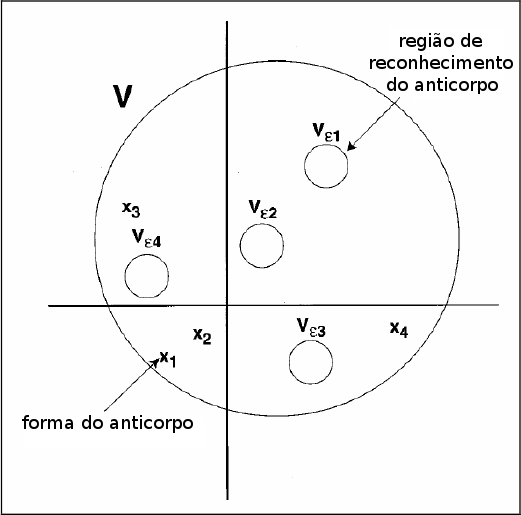
\includegraphics[width=0.75\textwidth]{img/space.png}
    \label{img:space}
\end{figure}

O espaço de formas é um hipercubo de volume V, e cada anticorpo é definido como uma área de reconhecimento nesse espaço ($\epsilon$). Na definição original, essas áreas de reconhecimento eram funções Gaussianas. A distância euclidiana entre \emph{ab} e \emph{ag} é considerada como a `afinidade' ou `medida de complementaridade'. Para isso, a natureza complementar dos anticorpos e antígenos é ignorada: uma ligação perfeita é considerada quando \emph{ab == ag}, ao contrário de \emph{ab != ag}. Anticorpos possuem uma hiper-região de reconhecimento, onde antígenos podem gerar uma resposta imune.

Uma crítica ao formalismo do espaço de formas foi feita em \citet{Carneiro1994}, destacando principalmente a simplicidade da abstração do espaço de estados e as limitações das funções de afinidade simples.

\section{Topologia de afinidade}

O objetivo de um anticorpo, no sistema imunológico, é maximizar a sua afinidade com um antígeno específico. Assim, a maturação de um anticorpo pode ser considerada também geometricamente como uma movimentação na superfície da função de afinidade para um antígeno específico \cite{Brownlee2007}.

Essa superfície teórica é geralmente considerada como contínua, e possui diversos ótimos locais, ou seja, um ponto com maior afinidade que seus vizinhos, mas que não é o ponto global com maior afinidade. Esse formalismo é útil na definição e formalização do processo de maturação por hipermutação dos anticorpos, parte principal dos algoritmos baseados na teoria da seleção clonal.

Os formalismos do espaço de formas e topologia de afinidades são a base da definição do espaço de formas binário usado na seleção negativa e nas redes imunológicas, das regiões e limiares de detecção nos algoritmos de mineração de dados e classificação, e da movimentação na topologia das funções de custo nos algoritmos de otimização.

A interpretação geométrica genérica proporcionada por esses dois formalismos constitui um \emph{framework} para a investigação de princípios imunológicos, não limitada aos problemas de reconhecimento de padrões.

\section{Considerações finais}

\citet{Dasgupta2010} observam que a maioria dos trabalhos recentes na área de Sistemas Imunológicos Artificiais têm seu foco em aplicações, ao invés de extensões, dos algoritmos existentes. Destacam também que existe uma sobreposição entre os modelos desses algoritmos e os evolucionários: os algoritmos de redes imunológicas artificiais, seleção clonal e genéticos têm componentes importantes em comum, como a clonagem, mutação e seleção.
